\documentclass[UTF8,a4paper]{ctexart}
%\usepackage[UTF8]{ctex}
\usepackage{graphicx}
\usepackage{url}
\usepackage{geometry}
\geometry{a4paper,scale=0.8}
\usepackage{setspace}
\setstretch{1.6}
\usepackage{listings}
\usepackage{xcolor}
\lstset{ 
  language=Python,  % 设置语言
  backgroundcolor=\color{lightgray},   % 背景颜色
  basicstyle=\ttfamily,    % 基本字体样式
  keywordstyle=\color{blue}, % 关键字颜色
  commentstyle=\color{gray}, % 注释颜色
  stringstyle=\color{red},   % 字符串颜色
  showspaces=false,          % 不显示空格
  showstringspaces=false,    % 字符串中的空格不显示
}

\begin{document}
\begin{sloppypar}


	\begin{center}
	
\includegraphics[width = 14cm]{picture/s1}

		\begin{fontsize}{60pt}{20pt}
			实验报告
		\end{fontsize}

		\bigskip
		\bigskip
		
		\begin{fontsize}{20pt}{20pt}
			\begin{flushright}
				—— 命令行环境与{\Huge python}基础及视觉应用的学习
			\end{flushright}
		\end{fontsize}
		
		\bigskip
		\bigskip
		\bigskip
		\bigskip
		\bigskip
		\bigskip
		\bigskip
		\bigskip
		\bigskip
		\bigskip
		\bigskip
		\bigskip
		\bigskip
		\bigskip
		\bigskip
		\bigskip
		
		\begin{fontsize}{25pt}{20pt}

			学号:
			\underline{{\huge 23060021010}}
			\bigskip
			\bigskip
			\bigskip
			\bigskip

			姓名:
			\underline{朱永基}
			\bigskip
			\bigskip
			\bigskip
			\bigskip

			班级:
			\underline{{\Huge 23}级工程管理}
				
		\end{fontsize}
	\end{center}
	\section{实验要求}
	\subsection{学习命令行环境的任务控制,终端多路复用,别名,配置文件,远端设备}
	\subsection{学习Python的基础入门及其视觉应用}
	\subsection{完成4个课堂练习与20个与命令行环境和Python有关的实例}

			\bigskip
			\bigskip
			\bigskip
			\bigskip

	\section{实验内容}
	\subsection{命令行环境的学习}
	\subsubsection{任务控制是指在命令行环境下管理和控制任务的执行状态(前台、后台、暂停等)。常用的任务控制命令有:\\Ctrl + C: 终止当前前台任务。\\Ctrl + Z: 暂停当前前台任务并将其放到后台。\\jobs: 列出当前所有的后台任务。\\fg [任务号]: 将后台任务恢复到前台执行。\\bg [任务号]: 在后台继续执行暂停的任务。\\kill [任务号或PID]: 终止指定的后台任务或进程。}
	\subsubsection{终端多路复用是指在一个终端中管理多个会话或窗口,允许用户在单一终端窗口中并行运行多个会话。最常用的多路复用工具包括tmux和screen。\\tmux new -s <session-name>: 创建一个新的 tmux 会话。\\Ctrl + b + d: 分离当前 tmux 会话(后台运行)。\\tmux ls: 列出所有 tmux 会话。\\tmux attach -t <session-name>: 恢复连接到指定的 tmux 会话。\\多路复用非常适合在远程会话中保持任务持续运行,即使断开连接,任务依然在后台执行。}
	\subsubsection{别名是为命令设置的快捷方式,用于简化复杂或常用命令的输入。可以通过在 shell 配置文件(如 ~/.bashrc 或 ~/.zshrc)中定义别名。\\配置文件用于设置命令行环境的个性化和自动化配置。常见的配置文件包括:\\~/.bashrc: Bash shell 的配置文件,通常用于定义别名、环境变量和自定义函数。\\~/.zshrc: Zsh shell 的配置文件,类似于 .bashrc。\\~/.bash\_profile 或 ~/.bash\_login: 在用户登录时执行的配置文件,通常用于设置环境变量。\\~/.vimrc: Vim 文本编辑器的配置文件,用于自定义编辑器的行为和外观。}
	
	\newpage
	
	\subsection{Python基础入门及计算机视觉应用}
	\subsubsection{Python 是一种高级的、解释型、面向对象的编程语言,由 Guido van Rossum 于 1991 年发布。由于其语法简洁、可读性强和庞大的标准库,Python 已成为应用广泛的编程语言,特别是在数据分析、人工智能、Web 开发、自动化等领域。}
	\subsubsection{python的特点:\\1.简洁易学:Python 语法简单,代码可读性强。它允许开发者用更少的代码完成同样的任务,因此非常适合初学者学习编程。\\2.跨平台:Python 是跨平台的,支持 Windows、MacOS、Linux 等操作系统,Python 代码在不同的操作系统上几乎不需要更改。\\3.解释型语言:Python 是解释型语言,代码可以逐行运行,无需编译,方便调试和快速开发。\\4.丰富的库和社区支持:Python 拥有丰富的标准库和第三方库,几乎可以实现任何应用场景的需求。比如科学计算的 NumPy 和 SciPy,数据分析的 Pandas,机器学习的 TensorFlow,Web 开发的 Django 等。\\5.强大的集成性:Python 能够轻松与其他语言(如 C、C++、Java)进行集成,支持扩展和调用外部库,适合多种应用开发。}
	\subsubsection{Python 在计算机视觉(Computer Vision, CV)领域具有广泛的应用,得益于其简洁的语法、强大的库支持以及活跃的社区。计算机视觉旨在让计算机能够“看见”并“理解”图像或视频内容,从而执行各种任务,如图像识别、对象检测、图像分割等。常用的Python计算机视觉库有OpenCV,TensorFlow和PyTorch等。}
	
	\newpage
	\graphicspath{{picture/}}

	
	\section{实例练习}
	\subsection{编写捕获SIGINT信号的py脚本}
	定义信号处理函数handler,将SIGINT信号处理程序设置为自定义的handler函数,实现了捕获此信号并控制程序行为。

	
	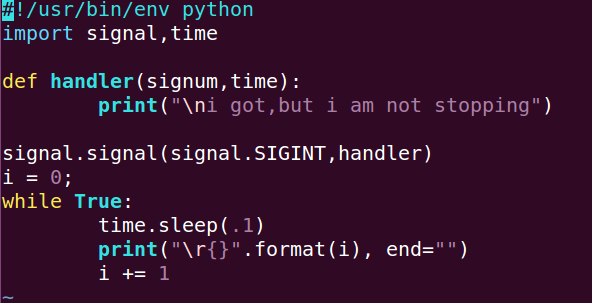
\includegraphics[width = 16cm]{1}
	
	\subsection{任务控制}
	输入Ctrl+c终止信号和Ctrl+z停止信号,终止信号被捕获
	
	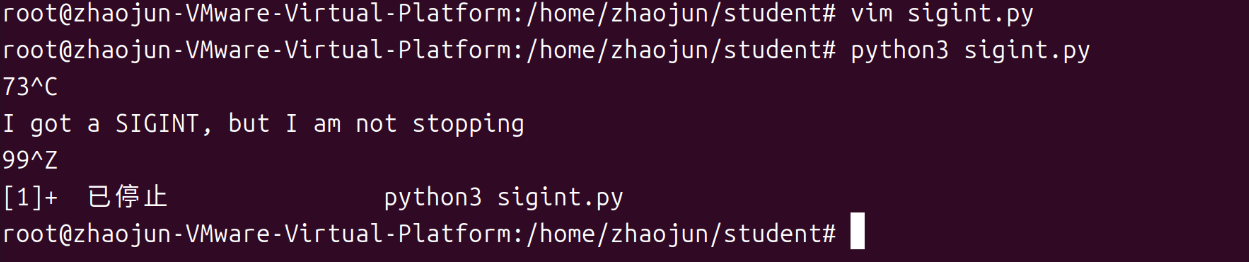
\includegraphics[width = 16cm]{2}
	
	\subsection{创建别名}
	利用alias命令,创建别名,mkd=mkdir
	
	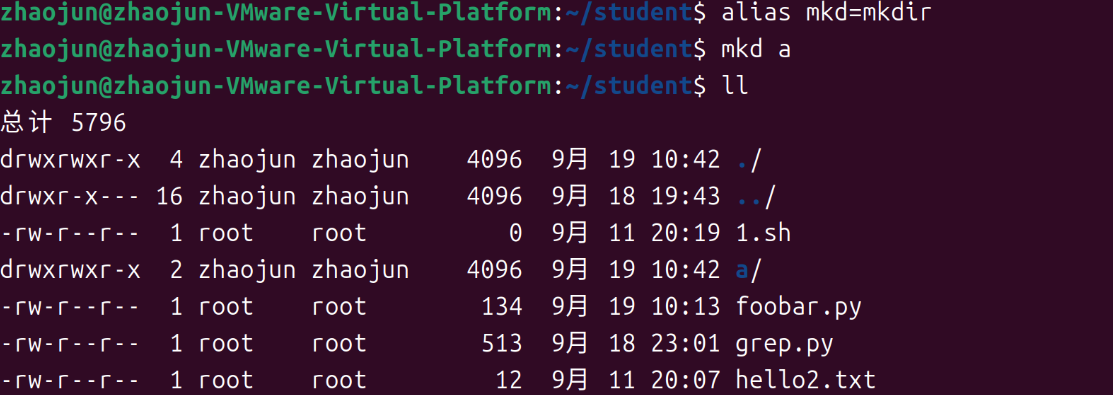
\includegraphics[width = 16cm]{3}
	
	\subsection{配置vimrc文件}
	配置~/.vimrc文件,设置语法高亮,显示行号,相对行号等,尤其相对行号方便快速移动到指定位置
	
	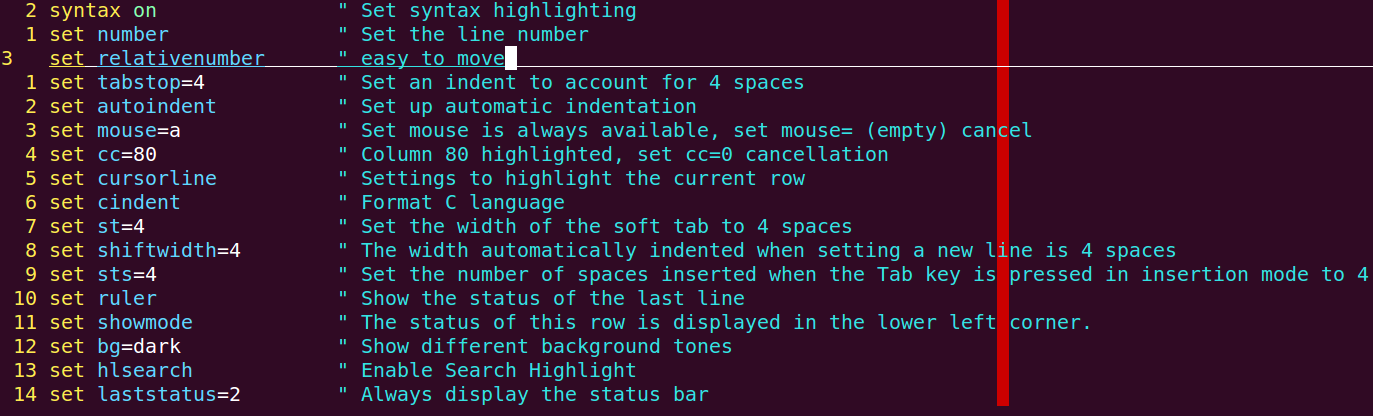
\includegraphics[width = 16cm]{4}
	
	\subsection{python计算日期}
	输入某年某月某日,判断这一天是这一年的第几天,代码及运行结果如下
	\begin{lstlisting}
year = int(input('year:\n'))
month = int(input('month:\n'))
day = int(input('day:\n'))

months = (0, 31, 59, 90, 120, 151, 181, 212, 243, 273, 304, 334)
if 0 < month <= 12:
    sum = months[month - 1]
else:
    print('data error')
sum += day
leap = 0
if (year % 400 == 0) or ((year % 4 == 0) and (year % 100 != 0)):
    leap = 1
if (leap == 1) and (month > 2):
    sum += 1
print('it is the %dth day.' % sum)
	\end{lstlisting}
	
	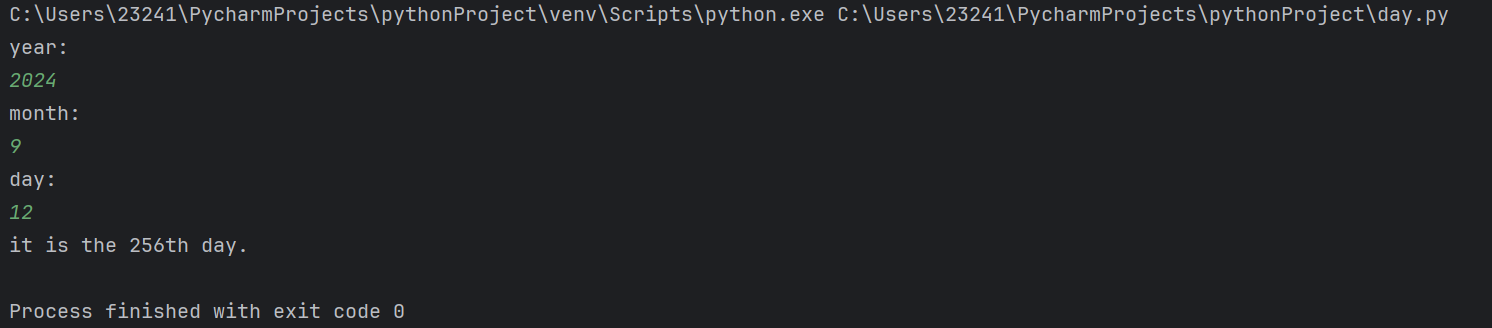
\includegraphics[width = 16cm]{5}
	
	\subsection{斐波那契数列}
	使用递归的方法输出斐波那契数列(展示第11个)
	\begin{lstlisting}
def fib(n):
    if n == 1 or n == 2:
        return 1
    return fib(n - 1) + fib(n - 2)

print(fib(11))
	\end{lstlisting}
	
	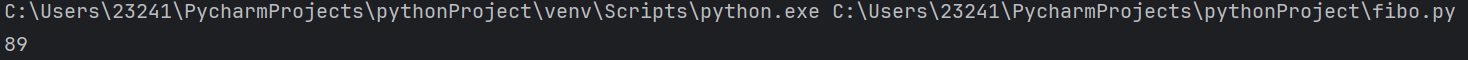
\includegraphics[width = 16cm]{6}
	
	\subsection{乘法口诀表}
	使用python的for循环输出乘法表
	\begin{lstlisting}
for i in range(1, 10):
    print()
    for j in range(1, i+1):
        print ("%d*%d=%d" % (i, j, i*j), end=" " )
	\end{lstlisting}
	
	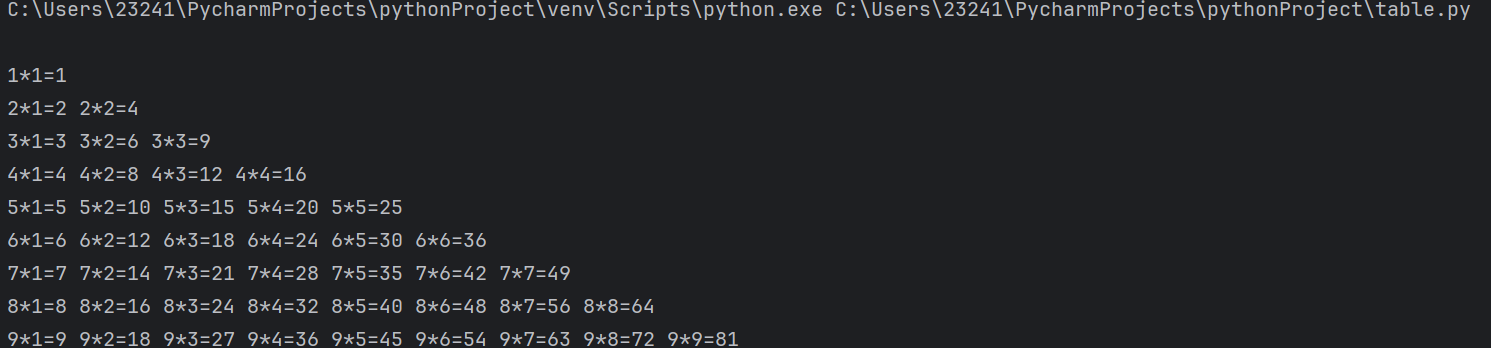
\includegraphics[width = 16cm]{7}
	
	\subsection{停顿输出}
	使用time模块的sleep()函数,实现停顿一秒再输出
	\begin{lstlisting}
import time

myD = {1: 'a', 2: 'b'}
for key, value in dict.items(myD):
    print(key, value)
    time.sleep(1)
    \end{lstlisting}
	
	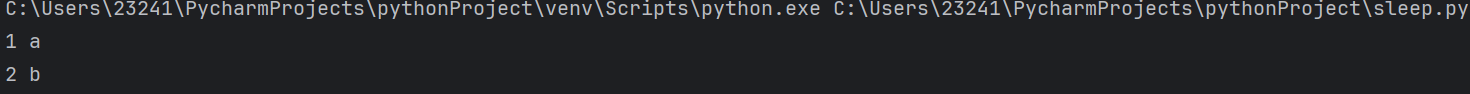
\includegraphics[width = 16cm]{8}
	
	\subsection{输出素数}
	输出201到301的素数,方法为分别用2到此数的平方根去除此数,若能整除则不是,反之为素数
	\begin{lstlisting}
h = 0
leap = 1
from math import sqrt
from sys import stdout
for m in range(201,301):
    k = int(sqrt(m + 1))
    for i in range(2,k + 1):
        if m % i == 0:
            leap = 0
            break
    if leap == 1:
        print ('%-4d' % m)
        h += 1
    leap = 1
print ('The total is %d' % h)
	\end{lstlisting}
	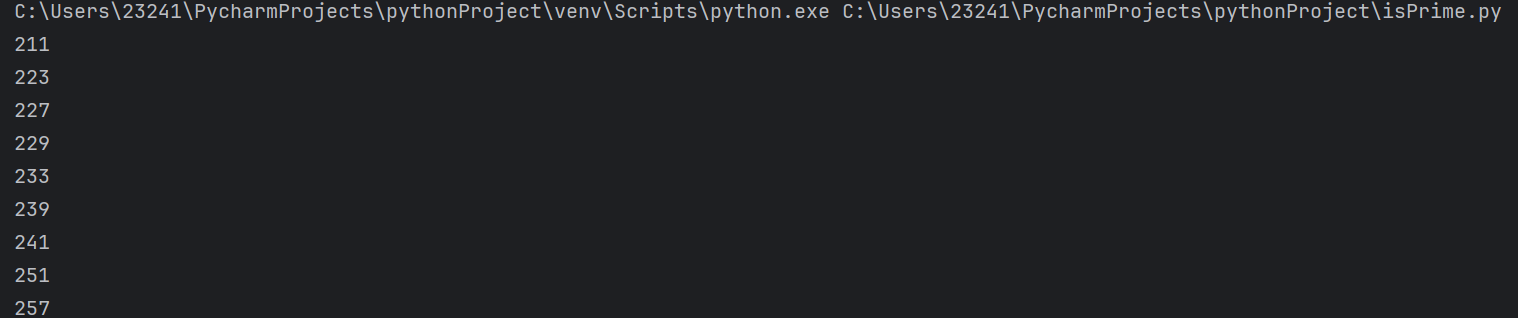
\includegraphics[width = 16cm]{9}
	
	\subsection{反顺序打印字符}
	利用递归函数调用方式反顺序输出
	\begin{lstlisting}
def output(s, l):
    if l == 0:
        return
    print(s[l - 1],end="")
    output(s, l - 1)

s = input('input:')
l = len(s)
output(s, l)
	\end{lstlisting}
	
\subsection{求最大公约数}
	采用欧几里得算法,计算最大公约数
\begin{lstlisting}
def gcd(a, b):
    while b:
        a, b = b, a % b
    return a

print(gcd(48, 18)) 
\end{lstlisting}


\subsection{判断回文字符串}
	利用python的切片操作,生成字符串的反转版本
\begin{lstlisting}
def is_palindrome(s):
    return s == s[::-1]

print(is_palindrome("racecar")) 
print(is_palindrome("hello"))

\end{lstlisting}

	
\subsection{列表去重}
	利用set的特性,和其高效的查找操作,检测重复的元素
\begin{lstlisting}
def remove_duplicates(lst):
    seen = set()
    unique_lst = []
    for item in lst:
        if item not in seen:
            unique_lst.append(item)
            seen.add(item)
    return unique_lst

print(remove_duplicates([1, 2, 3, 2, 1, 4, 5]))  

\end{lstlisting}

\subsection{统计字符出现次数}
	利用字典和其get()方法统计字符的出现次数
\begin{lstlisting}
def ccount(s):
    count = {}
    for char in s:
        count[char] = count.get(char, 0) + 1
    return count

print(ccount("hello world")) 

\end{lstlisting}

\subsection{冒泡排序}
	使用冒泡排序对数字进行排序
\begin{lstlisting}
def sort(lst):
    n = len(lst)
    for i in range(n):
        for j in range(0, n-i-1):
            if lst[j] > lst[j+1]:
                lst[j], lst[j+1] = lst[j+1], lst[j]
    return lst

print(sort([64, 34, 25, 12, 22, 11, 90]))
\end{lstlisting}

\subsection{合并两个有序列表}
	编写merge函数,合并两个有序列表并保持排序
\begin{lstlisting}
def merge(list1, list2):
    return sorted(list1 + list2)

print(merge([1, 3, 5], [2, 4, 6]))  
\end{lstlisting}

\subsection{连续子数组的最大和}
	使用卡丹算法,关键点在于判断对于当前元素,是加上前面的子数组后和最大,还是单独成为新的子数组最大,从而不断更新最大和
\begin{lstlisting}
def max_sum(nums):
    max_current = nums[0] 
    max_global = nums[0] 

    for i in range(1, len(nums)):
        max_current = max(nums[i], max_current + nums[i])

        if max_current > max_global:
            max_global = max_current

    return max_global

nums = [-2, 1, -3, 4, -1, 2, 1, -5, 4]
print(max_sum(nums))
\end{lstlisting}
	
	
	


	\section{实验收获与感悟}
	在学习命令行环境、任务控制、终端多路复用、别名、配置文件、远端设备与 Python 基础入门及其视觉应用后,我对工具的灵活性和高效性有了更深的理解。命令行是管理系统的关键,通过任务控制命令(如 `fg`、`bg`、`kill`),我学会了如何暂停、恢复和终止进程,体会到了在复杂系统中掌控任务的能力。同时,终端多路复用工具如 `tmux` 极大提升了操作效率,尤其在远程工作或系统管理中,它允许我在不中断工作的情况下同时管理多个会话,减少了上下文切换的时间浪费。\\
	\indent 别名和配置文件是日常操作效率的倍增器,通过自定义 `.bashrc` 或 `.vimrc` 文件,我能够简化复杂命令的执行并优化工作环境。在学习的过程中,我意识到一个高效的开发环境不仅仅依赖于工具的使用,更在于合理的配置和定制,这有助于长时间提高工作效率。与此同时,学习远程设备管理让我掌握了 SSH、SCP 等工具,能够无缝管理和维护远程设备,确保远程会话的安全性和稳定性。\\
	\indent 在Python 编程的学习中,我感受到了其简单易用性以及在多个领域的广泛应用,特别是在视觉应用方面,如使用 `matplotlib` 和 `OpenCV` 进行图像处理和数据可视化。通过掌握 Python 的基础数据结构和控制流,我不仅能够解决问题,还能在实践中理解编程与现实应用的结合。整体学习过程让我意识到,技术学习不仅仅是掌握工具,更是培养解决实际问题的能力,而实践在这个过程中起到了至关重要的作用。\\
	
	Github仓库链接:\url{https://github.com/zhaojun262510/program1}
	
\end{sloppypar}
\end{document}